\documentclass[twocolumn]{phdsymp} 

\usepackage{times}

\usepackage{tikz}
\usepackage{tikz-qtree}
\usetikzlibrary{arrows,positioning,calc} 

\def\BibTeX{{\rm B\kern-.05em{\sc i\kern-.025em b}\kern-.08em
    T\kern-.1667em\lower.7ex\hbox{E}\kern-.125emX}}

\newtheorem{theorem}{Theorem}


\usepackage{graphicx}

\usepackage{csquotes}
\usepackage[
    backend=biber,
    sortlocale=en_US
]{biblatex}

\addbibresource{references.bib}

\usepackage[utf8]{inputenc}
\usepackage[T1]{fontenc}

\usepackage{microtype}

\usepackage{caption}
\usepackage{subcaption}
\usepackage{multirow}

\usepackage{varioref}
\usepackage[plainpages=false,hidelinks]{hyperref}
\usepackage{cleveref}


\begin{document}

\title{From Metagenome to Metaproteome}

\author{Tom Naessens}

\supervisor{prof. dr. Peter Dawyndt, ir. Bart Mesuere \thanks{P.~Dawyndt and
B.~Mesuere are associated with the Computational Biology reseach group from the
Department of Applied Mathematics, Computer Science and Statistics, Ghent
University (UGent), Ghent, Belgium. E-mail: Peter.Dawyndt@UGent.be,
Bart.Mesuere@UGent.be.}}

\maketitle

\begin{abstract}
Comparing and analysing genomes is usually done using BLAST
\cite{altschul1990basic}. We propose the Unipept Metagenomics Analysis Pipeline,
a novel technique based on the conversion from metagenomics to metaproteomics
and back, which makes use of the Unipept Metaproteomics Analysis Pipeline
\cites{mesuere2012unipept, uniprot2014uniprot}. To achieve this, a more specific
version lowest common ancester (LCA) method is introduced for aggregating taxa. 
We also work out a proof of concept to modularise and extract the
current visualisations in Unipept into a standalone Unipept visualisation
framework, enabling users to inspect their data without uploading their data to
the Unipept web application.
\end{abstract}

\begin{keywords}
metagenomics, metaproteomics, unipept, benchmarking
\end{keywords}

\section{Introduction} 

The Unipept platform is developed to map diversity in large and complex
metaproteomic samples. The indexstructure of the underlying database has been
finetuned to allow quick retrieval of all proteins containing a certain tryptic
peptide. The taxon-specificity of a tryptic peptide can be determined based on
the taxonomy information from UniProt\cite{uniprot2014uniprot}. 

Taxon-specificity of the tryptic peptide is successively derived from these
occurrences using a novel lowest common ancestor approach that is robust against
taxonomic misarrangements, misidentifications, and inaccuracies.

We introduce a new pipeline, the Unipept Metagenomic Analysis Pipeline or UMAP
which allows the transformation of a metagenomics experiment into a
metaproteomics experiment, using the functionality of Unipept described above.
This pipeline is illustrated in \Vref{fig:van_naar}. For every DNA read in a
metagenomics sample, genes are extracted with
FragGeneScan\cite{rho2010fraggenescan} and are converted into proteins. These
proteins are then split into tryptic peptides. Then, the Unipept Metaproteomics
Analysis Pipeline is run to identify the consensus taxon for each tryptic
peptide. The resulting taxa are afterwards aggregated using the LCA* algorithm.

\begin{figure}[hbt]
	\centering
	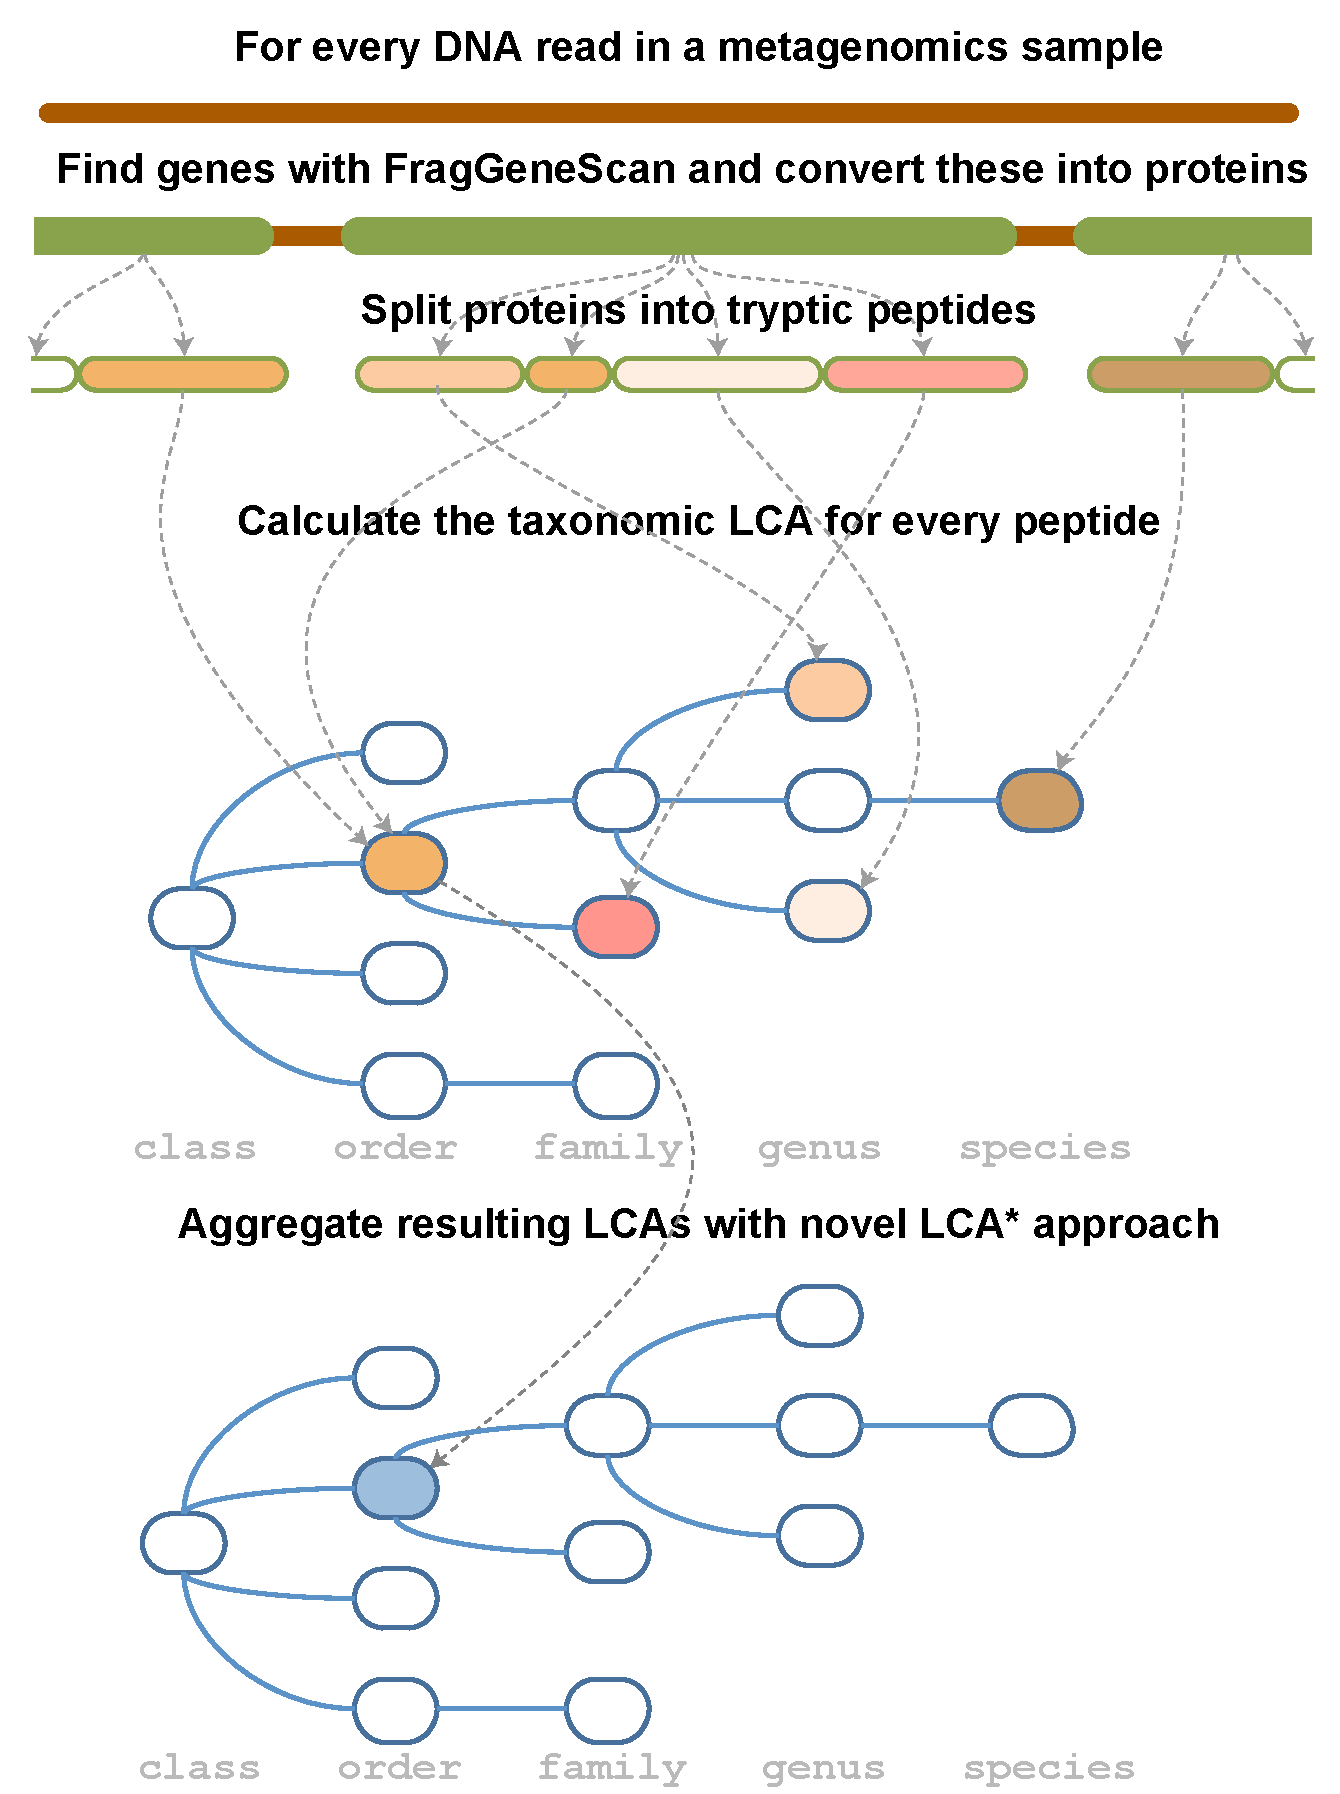
\includegraphics[width=\columnwidth]{includes/van_metagenoom_naar_metaproteoom.pdf}
	\caption{Illustration of the Unipept Metagenomics Analysis Pipeline. }
	\label{fig:van_naar}
\end{figure}


\section{LCA*} 

Unipept uses, as mentioned in the introduction, a robust implementation of the
lowest common ancestor algorithm which is used for the taxonomic identification
of one peptide. However, when the same algorithm is used to aggregate multiple
peptides from the same organism, it does not always yield the most specific
result.

Therefore, we introduce an adaptation of this algorithm which chooses more
specific identifications over less specific ones when the input taxa lie on the
same lineage. This new approach is illustrated in \Vref{fig:lca*example}.

\begin{figure}[hbt]
	\centering
    \begin{subfigure}{0.45\columnwidth}
        \centering
        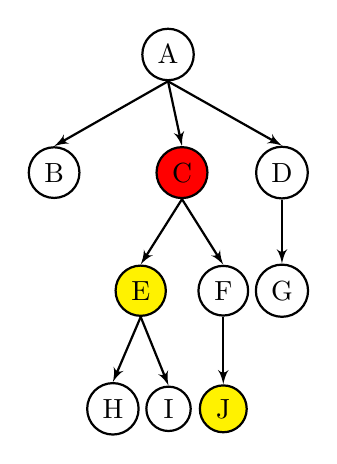
\begin{tikzpicture}[node distance=3cm, level distance=1.5cm,
            every node/.style={draw, thick, circle,inner sep=3pt},
            every path/.style={->, draw, thick, -latex'}]
        \Tree [. A 
                 [. B ]
                 [. \node[draw, fill=red]{C};
                    [.\node[draw, fill=yellow]{E};
                       [. H ]
                       [. I ]
                    ]
                    [. F
                       [. \node[draw, fill=yellow]{J}; ]
                    ] 
                 ]
                 [. D
                    [ . G ]
                 ] 
              ]
        \end{tikzpicture}
        \caption{}
        \label{tikz:lca*ej}
    \end{subfigure}
    \begin{subfigure}{0.45\columnwidth}
        \centering
        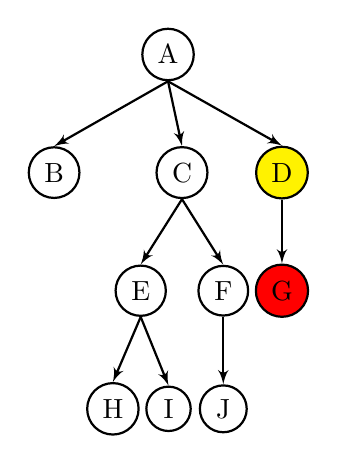
\begin{tikzpicture}[node distance=3cm, level distance=1.5cm,
            every node/.style={draw, thick, circle,inner sep=3pt},
            every path/.style={->, draw, thick, -latex'}]
        \Tree [. A 
                 [. B ]
                 [. C
                    [. E
                       [. H ]
                       [. I ]
                    ]
                    [. F
                       [. J ]
                    ] 
                 ]
                 [. \node[draw, fill=yellow]{D};
                    [ . \node[draw, fill=red]{G}; ]
                 ] 
              ]
        \end{tikzpicture}
        \caption{}
        \label{tikz:lca*dg}
    \end{subfigure}
    \caption{Examples of the novel LCA* calculation. On the left, LCA*(E, J) is
    calculated, yielding node C as a result. On the right, the LCA of node D and
    G is calculated, yielding the more specific result G instead of the regular
    result D.} 
    \label{fig:lca*example}
\end{figure}


\section{Benchmarking the Unipept Metagenomics Analysis Pipeline} 

To test the accuracy of the UMAP, we run two toolchains on three sorts of
genomes: \textit{i)} fully sequenced genomes, to be able to measure the accuracy
of the taxonomic identification, \textit{ii)} simulated unknown genomes (using a
kind of leave-one-out strategy), to measure the accuracy of the taxonomic
identification on genomes that have not been sequenced yet, and \textit{iii)}
genomes simulated with wgsim\cite{lh3/w4:online} based on fully sequenced
genomes of read length 250 with different read error percentages of 0, 1, 2 and
5, to measure the effect of read errors on the identification. The two
toolchains that were developed can be seen in \Vref{fig:abstractimage}. The left
toolchain is the UMAP itself, while the right toolchain introduces a filtering
step to simulate the unknown genomes.

\begin{figure}[hbt]
	\centering 
	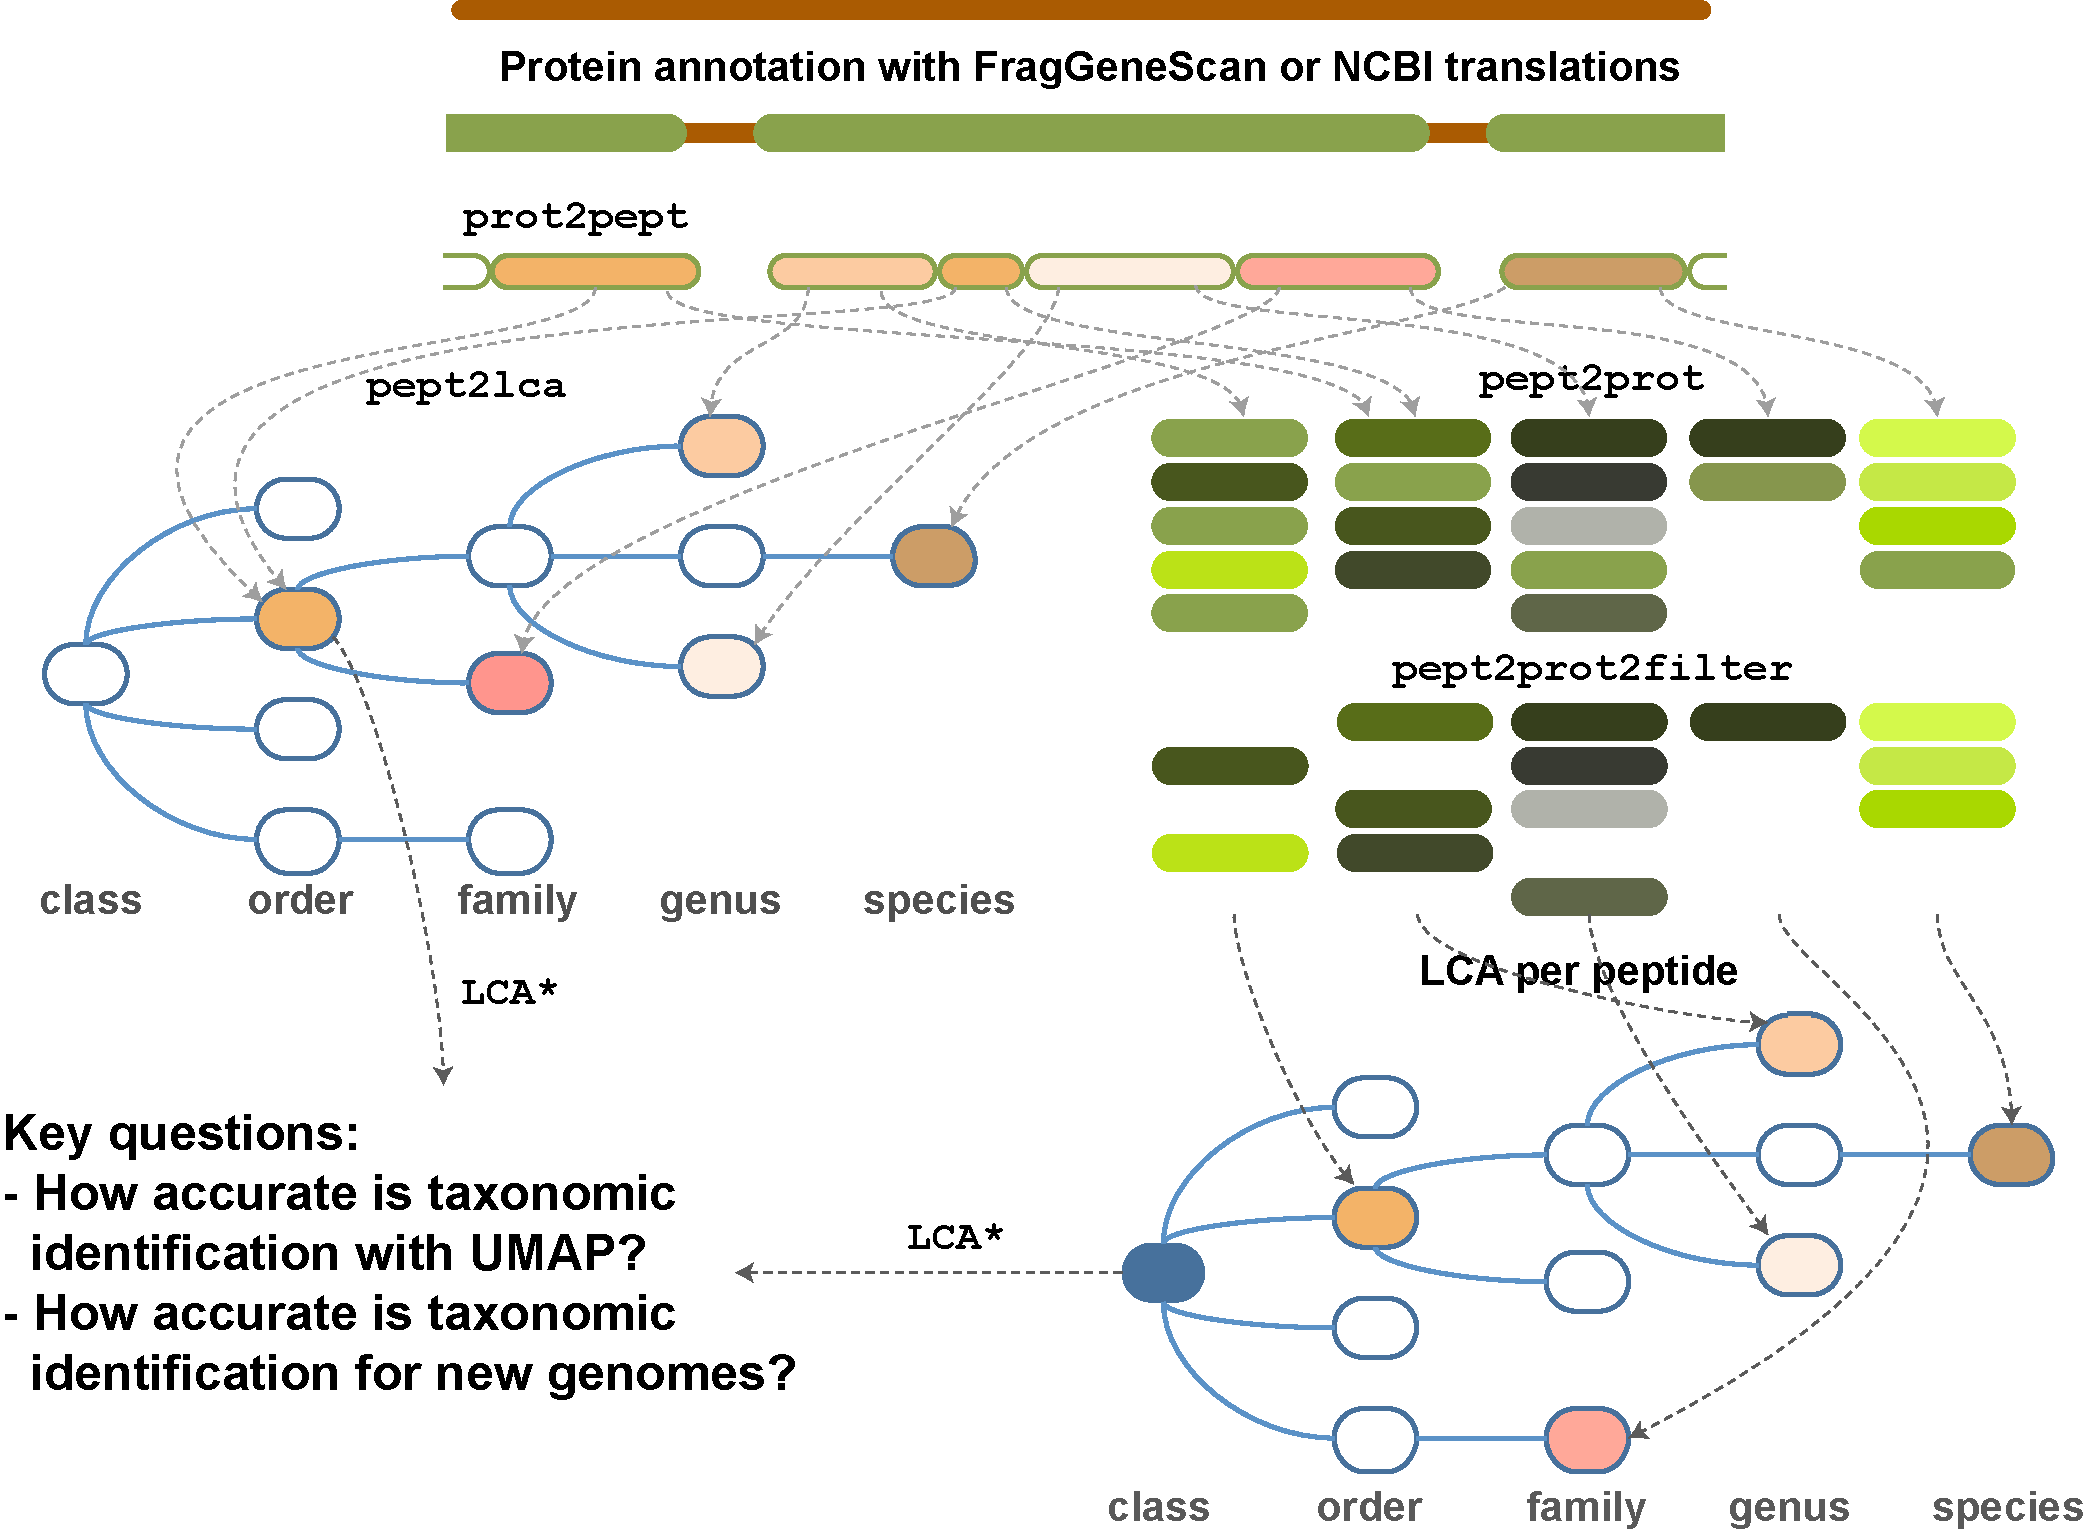
\includegraphics[width=\columnwidth]{includes/abstractimage.pdf}
	\caption{The two toolchains used in the benchmarking process. The left
	toolchain is the UMAP itself, while the right toolchain introduces a 
	filtering step to simulate the unknown genomes.}
	\label{fig:abstractimage}
\end{figure}

The UMAP has been found to identify fully sequenced genomes (\textit{i}) very
accurately with an average of 97\% of the proteins mapped to the species level.
When the toolchain is being run on simulated unknown genomes (\textit{ii}), a
shift in specificity to the lesser accurate levels is observed. 38\% of them
could still be mapped to the species level. When reads were introduced into the
genomes with wgsim (\textit{iii}), we notice less specific results as the error
percentage rises. The amount of proteins mapped to the species level drops just
below 50\% when the read error percentage crosses the level of 2\%.

The full results of the benchmarking process were published as a poster, shown
on the next page, which was presented during the annual BIG N2N symposium,
edition 2015\cite{BIGN3:online}.

\section{Unipept Visualisation Framework} 

We also set the first steps to create a modular and abstract visualisation
framework based on the current visualisations in the Unipept web application.
This visualisation framework allows users to inspect their results visually
and interactively, without having to enter their data in Unipept. As a proof of
concept, the treeview visualisation (as can be seen in \Vref{fig:treeviewarc})
was extracted from the Unipept code and put into a separate modular JavaScript
plugin.

\begin{figure}[hbt]
	\centering 
	\includegraphics[width=0.8\columnwidth]{includes/treeviewarc}
	\caption{Example of the treeview visualisation from Unipept}
	\label{fig:treeviewarc}
\end{figure}

\begin{figure*}[p]
	\centering
	\includegraphics[width=\textwidth]{includes/posterproject.pdf}
\end{figure*}

\nocite{*}

\printbibliography
\end{document}

%%%%%%%%%%%%%%%%%%%%%  End of phdsymp_sample2e.tex  %%%%%%%%%%%%%%%%%%%%%%%%%%%
